
% Chapter 2
\Chapter{MSSCopilot}{Generación de Código Automática}

\section{Objetivo de las prácticas}
El objetivo principal de las prácticas fue desarrollar una herramienta que permitiera a los usuarios generar código de manera automática. Esta herramienta, denominada MSSCopilot, debía ser capaz de generar código en C\# / Linq a partir de la base de código fuente existente en la compañía.

\begin{examplebox}

Un empleado le dice al MSSCopilot que desea obtener una lista con todos los Warehouses, el Copilot respondería con un código como el siguiente:

\begin{lstlisting}[language=C]
    using (var context = new MyContext())
    {
        var result = context.Warehouse.Select(x => x);
    }
    \end{lstlisting}
\end{examplebox}        

Durante el desarrollo del programa se elaboraron más funcionalidades de las previstas inicialmente como es la explicación de código, y otras más que se explicarán con mayor profundidad posteriormente.

El estado del proyecto al comenzar las prácticas estaba en una etapa inicial, lo que permitió un entendimiento más profundo del mismo y facilitó la integración de nuevas ideas y funcionalidades desde el principio. 

\section{Cosas}

Definir las tecnologías utilizadas en la realización del MSSCopilot resulta complicado porque como se ha comentado en la sección \ref{sec:contexto}, aunque se trate de desarrollar un producto de software, ha sido un proyecto en el que, por la naturaleza de la IA, que sigue siendo un sector de tecnologías emergentes, las directrices a seguir no son tan claras. Debido a esto, gran parte del proyecto ha consistido en un proceso de investigación en el que se han utilizado tecnologías y técnicas que, con el tiempo, se han descartado en favor de otras opciones mejores a medida que se identificaban.

Los LLM son un tipo de modelo de inteligencia artificial diseñado para comprender y generar texto, como es el famoso GPT, para este proyecto se ha utilizado Ollama.

En la descripción de las prácticas una de las tareas fundamentales era diseñar y entrenar el sistema a partir de la base de código fuente existente en la
compañía. Para entrenar un LLM con información nueva hay dos opciones:
\begin{itemize}
    \item Ajustar el modelo preentrenado utilizando un cojunto de datos más pequeño y específico, proceso conocido como \bold{Fine-tuning.}
    \item Convertir palabras, frases o textos completos en vectores numéricos. Estos \bold{Embeddings} capturan el significado y las relaciones semánticas del texto. Se pueden convertir las preguntas del usuario en embeddings y compararlos con los embeddings de la información que tenemos almacenada en una BDD, y si ambos tienen x similitud darle esa información al LLM en tiempo real para que responda con nuestra información.
\end{itemize}

En resumen, en la primera opción ponemos al modelo a estudiar los conocimientos nuevos generando así un nuevo modelo, y en la segunda opción es como si el modelo para cada pregunta, consultase en un diccionario/libro con respuestas, buscando la que más se parezca a la pregunta del usuario. 

Inicialmente se optó por utilizar Embeddings, usando SQLite para la BDD y C\# por compatibilidad con toda la infraestructura de la empresa, permitiendo el poder integrar a futuro esta utilidad de asistente de código a todos los servicios que ofrecen.

La base de datos contenía previamente querys correctamente escritas en C\# junto con su respectiva descripción, y el embedding asociado, esto se descartó posteriormente ya que no era viable para la empresa ponerse a generar querys con descripciones para cada casuística, y en versiones posteriores se optaría por pasarle el contenido de las tablas.

\newpage
Dicha comparación que se realiza entre Embeddings de la pregunta del usuario y la BDD se tuvo que implementar en código, se implementó tanto la similitud coseno como la euclídea:


\begin{figure}[htbp]
    \centering
    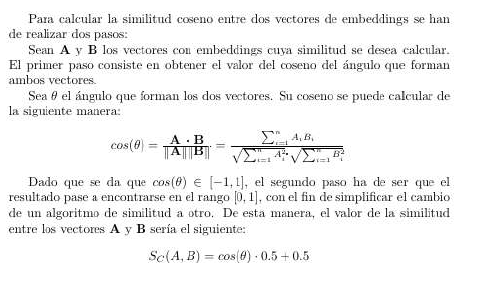
\includegraphics[width=0.8\textwidth]{Chapters/cap4.PNG}
    \label{fig:mi_imagen}
\end{figure}

\begin{figure}[htbp]
    \centering
    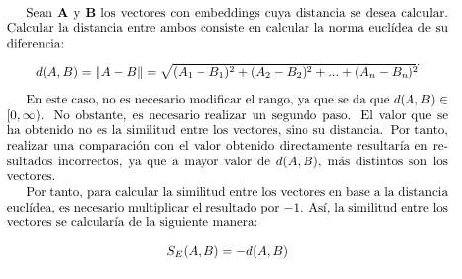
\includegraphics[width=0.8\textwidth]{Chapters/cap5.PNG}
    \label{fig:mi_imagen2}
\end{figure}
